\tikzset{>=latex} % for LaTeX arrow head
\colorlet{myblue}{black!40!blue}
\colorlet{myred}{black!40!red}
\colorlet{vcol}{green!50!black}
\colorlet{Ecol}{orange!90!black}
\colorlet{EVcol}{orange!80!black!60}
\colorlet{Bcol}{violet!90}

% Electromagnetic wave - colored





% Electromagnetic wave SHORT - colored


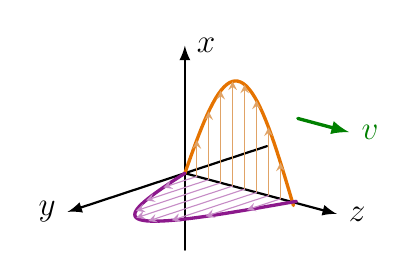
\begin{tikzpicture}[x=(-15:0.9), y=(90:0.9), z=(-150:1.1),
                    line cap=round, line join=round,
                    axis/.style={black, thick,->},
                    vector/.style={>=stealth,->}]
  \large
  \def\A{1.5}
  \def\ymax{1.8}
  \def\nNodes{1} % use even number
  \def\nVectorsPerNode{8}
  \def\N{\nNodes*40}
  \def\xmax{\nNodes*pi/2*1.01}
  \pgfmathsetmacro\nVectors{(\nVectorsPerNode+1)*\nNodes}
  
  % MAIN AXES
  \draw[axis] (0,0,0) -- ++(\xmax*1.4,0,0) node[right] {$z$};
  \draw[axis] (0,-\ymax*0.6,0) -- (0,\ymax,0) node[right] {$x$};
  \draw[axis] (0,0,-\ymax*0.7) -- (0,0,\ymax) node[left] {$y$};
  
  \draw[Ecol,very thick,variable=\t,domain=0:pi/2*1.01,samples=40]
    plot (\t,{\A*sin(\t*360/pi)},0);
  \foreach \k [evaluate={\t=\k*pi/2/(\nVectorsPerNode+1);
                         \angle=\k*90/(\nVectorsPerNode+1);}]
              in {1,...,\nVectorsPerNode}{
    \draw[vector,EVcol]  (\t,0,0) -- ++(0,{\A*sin(2*\angle)},0);
  }
  \draw[Bcol,very thick,variable=\t,domain=0:pi/2*1.01,samples=40]
    plot (\t,0,{\A*sin(\t*360/pi)});
  \foreach \k [evaluate={\t=\k*pi/2/(\nVectorsPerNode+1);
                         \angle=\k*90/(\nVectorsPerNode+1);}]
              in {1,...,\nVectorsPerNode}{
    \draw[vector,Bcol!50]  (\t,0,0) -- ++(0,0,{\A*sin(2*\angle)});
  }
  
  % VECTOR
  \draw[->,very thick,vcol] (\A*1.1,\A*0.8,0) --++ (\A*0.5,0,0) node[right] {$\vb{v}$};
  
\end{tikzpicture}
